% IEEE conference writing draft. Verify the selected venue's review rules.
\documentclass[conference]{IEEEtran}
\usepackage[T1]{fontenc}
\usepackage[utf8]{inputenc}
\usepackage{amsmath,amssymb,booktabs,array,graphicx}
\usepackage[numbers,sort&compress]{natbib}
\usepackage{microtype}
\usepackage[hidelinks]{hyperref}
\setlength{\emergencystretch}{2em}
\newcommand{\tightlist}{\setlength{\itemsep}{0pt}\setlength{\parskip}{0pt}}
\providecommand{\pandocbounded}[1]{#1}
\begin{document}
\title{Shardwise: Measurement Pitfalls in Repartitioning Small CPU
Language Models}
\author{\IEEEauthorblockN{Anonymous Authors}}
\maketitle
\begin{abstract}
Splitting a language model that fits on each available machine creates a
serving choice rather than a capacity requirement. We study that choice
with Shardwise, a CPU runtime for contiguous-layer inference,
repartitioning, and replay recovery. An audit of 65 two-VM Qwen3-0.6B
runs shows that a 25\% gain during an injected CPU fault shrinks to
about 5--7\% over the complete run, while adaptation under injected link
delay loses about 6--8\%. A migration payback gate demonstrates no
advantage over hysteresis. We distinguish ideal capacity from
finite-session completion, give a three-worker counterexample to a
saturation heuristic, and implement an exact finite-concurrency envelope
planner. Separate single-repetition local checks compare pipeline,
replica, and unsplit execution across concurrency one to eight; they
establish functional coverage, not statistical superiority. Eighteen
position-controlled recovery cases preserve exact greedy outputs while
exposing token stalls of up to about ten seconds. A packaged application
demonstrates real inference, worker-stop recovery, and restored
placement through a browser interface. The results identify baseline
choice, transition accounting, and telemetry contamination as central
limits on conclusions drawn from small deployments.
\end{abstract}
\begin{IEEEkeywords}
LLM inference, pipeline parallelism, CPU serving, performance
measurement, recovery
\end{IEEEkeywords}
\hypertarget{introduction}{%
\section{Introduction}\label{introduction}}

A small language model can fit on each of several available machines. In
this setting, splitting layers is one serving option; complete-model
replication is another. Independent requests can overlap across pipeline
stages, while a single autoregressive request traverses every active
stage for each token. Moving layer boundaries introduces another
tradeoff: a better steady-state placement may arrive too late to repay
its reconfiguration cost.

Shardwise provides a compact implementation in which these costs can be
inspected. A Go controller places contiguous decoder-layer ranges;
Python workers execute them over gRPC; a router tracks independent
request histories and rebuilds their KV caches after a generation
change. Its techniques are established. The question here is how
measurement and baseline choices affect the conclusions drawn from a
small running service.

The original two-VM record contains 65 runs and 939 requests. We audited
that record without changing the raw data. Its most useful findings are
negative: whole-run adaptation gains are smaller than fault-phase gains;
moving under delay hurts; the transition-cost gate does not outperform a
simpler policy in the observed medians; and a remaining-work horizon
does not describe a service whose clients keep admitting new requests.
One-thread whole-model execution also leaves a central baseline question
unresolved: if the model fits on both machines, why not replicate it?

We examine that question with separate local baseline checks, while
keeping one-repetition validation distinct from the unfinished repeated
study. The completed contributions are (i) an audited empirical study
with explicit claim boundaries, (ii) position-controlled replay checks
and queue instrumentation, and (iii) a corrected planner for the ideal
finite-concurrency envelope. An installable application makes the
execution and recovery behavior visible. Exact optimization of this
model does not imply optimal placement on the real runtime. We do not
claim a new general migration, recovery, or partitioning principle.

\hypertarget{related-work}{%
\section{Related Work}\label{related-work}}

Pipeline parallelism and contiguous placement precede this system
\citep{huang2019gpipe, narayanan2019pipedream, bokhari1988partitioning}.
EdgeShard separates sequential latency from pipelined throughput and
uses dynamic programming with device and memory constraints
\citep{edgeshard2025}. Petals demonstrates distributed block serving and
recovery on consumer devices \citep{borzunov2023petals}. Those systems
address broader capacity aggregation than the small model studied here.

Migration payback is established. DiSCo admits generation handover using
remaining decode savings and migration overhead; STAR filters migrations
that cannot amortize their cost \citep{sun-etal-2025-disco, star2026}.
ServerlessLLM reconstructs state from token history
\citep{fu2024serverlessllm}. SpotServe combines workload-aware serving,
migration, re-parallelization and preemption recovery
\citep{miao2023spotserve}. These capabilities prevent presenting their
combination as an independent novelty claim.

DynoPipe jointly considers workload, queueing, compute, network
conditions and pipeline switching in a heterogeneous edge/cloud GPU
system \citep{lin2026dynopipe}. Its RTX 3090 edge and A40 cloud
deployment differs from our CPU testbed. FlexPipe adapts pipeline
granularity to request patterns and maintains cache consistency during
refactoring \citep{lin2026flexpipe}. Shardwise's distinction is
narrower: an inspectable CPU implementation and evidence about short-run
disruption, baseline dispatch, and misleading telemetry. No matched
experiment with these prior systems was performed.

An August 2026 preprint examines pre-compiled OpenVINO pipeline shards
and multiuser interleaving on Intel AI PCs
\citep{berenbaum2026precompiled}. It provides additional
commodity-device context; we do not treat it as verified peer-reviewed
acceptance or a matched comparison with our runtime.

Performance methodology calls for resource-matched alternatives,
variability and a clear analysis unit
\citep{jain1991art, hoefler2015benchmarking}. We use runs as units,
retain failures, and report phase and whole-run metrics separately.
Requests within a run do not increase the independent sample size.

\hypertarget{runtime-and-decision-model}{%
\section{Runtime and Decision Model}\label{runtime-and-decision-model}}

\hypertarget{execution-and-recovery}{%
\subsection{Execution and recovery}\label{execution-and-recovery}}

Workers hold half-open ranges of decoder layers. The first active stage
embeds tokens; the last applies normalization and the output head. Each
worker serializes compute with one lock. Independent request threads can
overlap between stages, but there is no continuous batching or
speculative decoding. The router passes activations through an ordered
chain and receives the greedy next token. In cached mode, later steps
send one position per request.

Every assignment has a generation. Workers reject a forward from another
generation. On a relayout, missing cache, or unreachable worker, the
router obtains the available layout and replays the entire accumulated
token history under a fresh request identifier. Already accepted output
tokens remain in the history. This mechanism requires enough surviving
memory to hold the assigned model; it does not protect the router or
controller machine.

Node agents report compute-speed and network observations to the
controller. Kernel TCP telemetry and application timing are separate
sources. The latter historically used RPC time minus worker compute
time, which also prices time waiting for the worker. The revision
exposes compute-lock wait separately and offers an opt-in
queue-corrected residual. That remaining residual includes
serialization, dispatch and transport; it is not pure network RTT.

\hypertarget{placement-and-the-concurrency-qualification}{%
\subsection{Placement and the concurrency
qualification}\label{placement-and-the-concurrency-qualification}}

For a nonempty worker range \([a,b)\), the cost model prices layer
compute, endpoint modules and the link into that worker:

\[d_i(a,b)=\frac{(b-a)c(C)+e\mathbf{1}_{a=0}+h\mathbf{1}_{b=L}}{s_i}
 +\ell_i. \tag{1}\]

The local worker has zero link term. Empty workers are skipped and cost
zero. The model assumes fixed worker order, additive stage costs, and no
explicit memory constraint. Measured context costs interpolate \(c(C)\).
Sum placement minimizes \(P=\sum_i d_i\); saturated throughput placement
minimizes \(B=\max_i d_i\). The ordered DP combines a prefix optimum
with each possible last range, using addition for \(P\) and maximum for
\(B\), in \(O(WL^2)\) time.

For \(Q\) non-speculative requests, ideal aggregate throughput obeys

\[X_Q\le\min(1/B,Q/P),\qquad j_Q=\max(B,P/Q). \tag{2}\]

Each token needs service at every stage, giving the bottleneck bound;
the closed network has at least \(P\) cycle time, giving the
request-count bound through Little's law
\citep{little1961proof, reiser1980mva}. These are capacity bounds, not
achievable-throughput predictions. Prefill, queues, interpreter overhead
and changing request lengths remain outside the envelope.

The historical automatic policy selected sum at \(Q\le1\) and bottleneck
otherwise. This two-worker heuristic does not generalize. Nine unit-cost
layers on three equal workers with unit costs into remote nonempty
workers give a minimum bottleneck \(B=4\) with \(P=11\). At \(Q=2\), its
envelope cost is 5.5. Two active stages can instead give \(B=5,P=10\),
for cost 5.

The revised automatic planner minimizes \(j_Q\) directly. It enumerates
possible stage-cost caps \(b\) and runs a sum DP restricted to stages no
greater than \(b\). The least achievable sum \(P(b)\) decreases as the
cap increases. Before the first crossing \(b\ge P(b)/Q\), the score is
\(P(b)/Q\); after it, the score is \(b\). Comparing the crossing and its
predecessor yields the exact optimum. Binary search requires
\(O(\log(WL^2))\) constrained DPs, each \(O(WL^2)\), after sorting the
possible caps. Exhaustive enumeration of 1,000 small random instances
checks heterogeneity, empty stages, endpoints and concurrency. The
historical results below use the original planner.

\hypertarget{payback-and-finite-cohorts}{%
\subsection{Payback and finite
cohorts}\label{payback-and-finite-cohorts}}

Voluntary moves first pass an improvement threshold and cooldown. The
historical gate estimates transition time as

\[T=F+CpL, \tag{3}\]

with fixed load/orchestration cost \(F\), configured context \(C\), and
replay cost \(p\) per token-layer. It prices the entire chain, including
unmoved layers. However, the configured \(C\) does not sum simultaneous
request histories. The revision offers a live-context forecast
\(F+pL\sum_r C_r\), where each \(C_r\) contains prompt and accepted
output tokens. This estimates serial replay work; overlap, weights,
serialization and orchestration still require calibration. Unavailable
live-context telemetry holds voluntary moves but permits recovery.

For positive current and candidate token costs \(j_c>j_n\), horizon
\(H\) and relative capacity margin \(m\ge0\), the historical fluid gate
accepts when

\[\frac{(H-T)_+}{j_n}>(1+m)\frac{H}{j_c}. \tag{4}\]

Multiplying positive denominators shows that, for \(T>0\), acceptance is
equivalent to \(\Delta_m=j_c-(1+m)j_n>0\) and \(H>Tj_c/\Delta_m\).
Capping the horizon at \(\min(H,Rj_c)\) additionally requires
\(R>T/\Delta_m\). This is an algebraic statement about the chosen
capacity surrogate. It is not a necessary-and-sufficient guarantee for
real session completion. A finite cohort cannot produce more than its
\(R\) remaining tokens; concurrency also decreases as requests finish.
For constant costs, the zero-margin makespan comparison is
\(T+Rj_n<Rj_c\). A completion-time margin would require a separately
stated condition, such as \((1+m)(T+Rj_n)<Rj_c\).

\hypertarget{experimental-method}{%
\section{Experimental Method}\label{experimental-method}}

\hypertarget{historical-two-vm-evidence}{%
\subsection{Historical two-VM
evidence}\label{historical-two-vm-evidence}}

The audited record uses Qwen3-0.6B, 28 layers, FP32 CPU execution and KV
caching on two Azure VMs with two vCPUs and about 8 GiB each. One worker
thread per machine is used. The coordinator hosts the controller, router
and one worker. The matrices comprise 20 objective runs, 12 demand runs,
30 adaptation runs and three single-device runs. The total is 65 runs,
939 requests and 19 recorded request failures. Distinct source snapshots
are retained and matrices are not pooled. Raw host labels differ from
the manuscript labels and are documented in the artifact.

Objective runs compare sum and bottleneck placement at concurrency one
and two, with stable links or 120 ms injected delay. Adaptation compares
static, hysteresis, gate and forced-gate arms under CPU quota, link
delay or worker loss. The demand matrix compares fixed throughput
placement and historical automatic placement with fixed or
remaining-work horizons. These comparisons have only two or three
independent repetitions per condition.

Whole-run throughput divides successful output tokens by elapsed time
through the last request's completion, including drain and failures.
Historical fault-phase throughput assigns tokens by request completion
within the logged fault window, not by streamed token timestamps. This
convention can move work across phase boundaries. Median request latency
and router TTFT are supporting metrics; TTFT does not measure client
streaming delivery.

\hypertarget{local-validation-and-its-analysis-unit}{%
\subsection{Local validation and its analysis
unit}\label{local-validation-and-its-analysis-unit}}

The local baseline checks form an additional evidence stratum. All four
arms use the same cached FP32 Qwen3-0.6B model, prompts, greedy output,
worker backend and HTTP/gRPC path. They are one-thread unsplit serving,
two-thread unsplit serving, two complete-model one-thread replicas, and
two one-thread pipeline workers with fixed 18/10 placement. Two host
CPUs are reserved for inference; the one-thread unsplit arm leaves one
unused. Two other host CPUs provide coordination. Replicas reserve the
first available endpoint for an entire request, including dispatch wait
in client latency.

On an AMD EPYC 7763 host, one randomized restart block covers contexts
of 32 and 128 tokens, 16 output tokens, and concurrency \(Q=1,2,4,8\).
Each run serves at least four requests and at least as many as its
concurrency. The 32 runs contain 160 requests. The driver saves prompts,
reference outputs, model revision, package versions, source hashes, CPU
affinities and process memory. Every successful sequence is checked
against unsplit Hugging Face greedy output. The model revision is
\texttt{c1899de289a04d12100db370d81485cdf75e47ca}; the research
environment uses PyTorch 2.8.0 and Transformers 4.57.1. Inputs are
seeded pseudorandom token IDs, not a natural-language task suite. They
control length and support exact reference checks, but do not establish
answer quality.

A separate one-block, three-worker check reserves three inference CPUs
and one coordination CPU. It measures a context-256 component profile
before comparing three-thread unsplit execution, three whole-model
replicas, bottleneck placement, and finite-concurrency capacity
placement at \(Q=1,2,4,8\), with 32 output tokens. Layouts are fixed for
each concurrency; this is not an adaptive-controller trial. Its 16 runs
contain 80 requests. A configured 1 ms coefficient into remote stages
models loopback placement cost; it is not a measured WAN delay. Empty
stages launch no worker. Workers load their checkpoints sequentially to
avoid simultaneous full-model loading.

These local matrices have only one repetition per condition. We report
observations without confidence intervals or statistical significance
claims. Requests within a run are not independent repetitions. Earlier
ten-block campaigns stopped after 129/320 and 37/320 runs on different
CPUs; those partial campaigns, their pilots and the present checks
remain separate. The repeated study and optimized external-engine
baseline are unfinished. Single-host loopback execution does not
reproduce physical heterogeneity or Azure links.

Recovery checks manually inject relayout, remote-worker loss, or
remote-worker restart at accepted-token positions 1, 4 and 12, with one
and two active requests. Actual Qwen3 worker processes and gRPC are
used; the survivor loads the full model after loss. Eighteen cases check
27 outputs of 16 tokens each. They validate replay sequencing and
internal stalls, not heartbeat detection, controller response,
coordinator loss or streamed HTTP delivery.

\hypertarget{results}{%
\section{Results}\label{results}}

\hypertarget{objective-choice-helps-an-internal-baseline}{%
\subsection{Objective choice helps an internal
baseline}\label{objective-choice-helps-an-internal-baseline}}

With two stable concurrent requests, historical bottleneck placement
achieves 7.303 versus 4.046 tokens/s for sum placement, an 80.5\% gain.
With one request, they achieve 3.875 and 4.029 tokens/s. Under injected
delay at concurrency one, sum placement achieves 4.001 versus 2.419
tokens/s: 65.4\% higher throughput, or a 39.5\% loss in the reverse
comparison. Median completion time falls from 12.531 to 8.012 s, a
36.1\% reduction.

\begin{figure}[t]
\centering
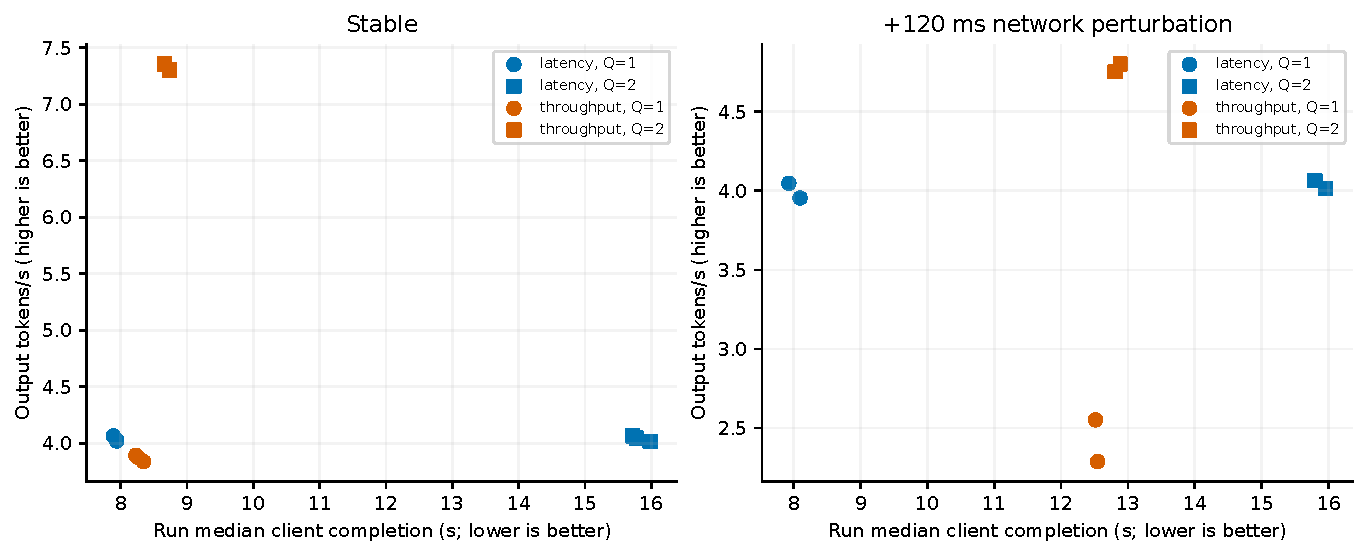
\includegraphics[width=\linewidth]{figures/objective-frontier.pdf}
\caption{Historical objective runs on two VMs. Each point is a run. Whole-run throughput and completion include drain. Sum and bottleneck arms activate different amounts of compute; this is not a replica comparison.}
\label{fig:objectives}
\end{figure}

These results show that objective choice matters inside this runtime.
They also compare different amounts of active compute: sum placement can
put the whole model on one worker, while bottleneck placement activates
both. They therefore do not establish superiority over resource-matched
serving.

\hypertarget{the-gate-has-no-demonstrated-benefit-over-hysteresis}{%
\subsection{The gate has no demonstrated benefit over
hysteresis}\label{the-gate-has-no-demonstrated-benefit-over-hysteresis}}

Under CPU slowdown, hysteresis achieves 5.269 versus 4.215 fault-phase
tokens/s for static placement, a 25.0\% gain. Whole-run throughput
changes from 5.744 to 6.133, only 6.8\%. The gate achieves 6.041
whole-run tokens/s. Under delay, static achieves 6.554, hysteresis 6.131
and gate 6.055 tokens/s. Both adaptive arms lose about 6--8\% over the
complete run despite similar fault-phase throughput. Under worker loss,
gate and hysteresis restore service with no failed requests; static
records 19. The fault-blind static comparison does not establish better
availability than replication or another recovery policy.

\begin{table}[t]
\centering\small
\caption{Historical whole-run throughput medians (tokens/s). Independent repetitions per arm: three for CPU and delay; two for loss. The differences do not establish statistical significance.}
\begin{tabular}{lrrr}
\toprule Condition & Static & Hysteresis & Gate\\
\midrule CPU slowdown & 5.744 & 6.133 & 6.041\\
Link delay & 6.554 & 6.131 & 6.055\\
Worker loss & 3.271 & 5.443 & 5.409\\
\bottomrule
\end{tabular}
\label{tab:adaptation}
\end{table}

No observed median demonstrates a gate advantage. With only two or three
repetitions, the small differences between gate and hysteresis are not
evidence of a statistically established loss either. The defensible
finding is that adding a reasonable cost gate did not demonstrate better
serving in this record.

At concurrency two in the demand matrix, fixed throughput placement
achieves 7.830 tokens/s, historical automatic fixed-horizon placement
5.944, and automatic remaining-work placement 5.729. Starting with the
wrong layout and waiting through cooldown can dominate the later policy
choice. Remaining-work admission also renews whenever a closed-loop
client begins another request. A present-cohort budget and a forecast of
continuing demand are different quantities.

\hypertarget{forecasts-and-telemetry-need-careful-denominators}{%
\subsection{Forecasts and telemetry need careful
denominators}\label{forecasts-and-telemetry-need-careful-denominators}}

Historical request disruptions grouped with executed decisions yield 34
estimated transitions. Compute-fault disruptions average 5,382 ms
against a 3,054 ms forecast; network-fault disruptions average 3,948 ms.
Measurements exceed forecast by 76.2\% and 29.2\%. Equivalently, the
forecast is 43.3\% and 22.6\% below measurement. These percentages use
different denominators and must not be interchanged. Historical grouping
lacked explicit transition IDs; the 34 groups are not a directly logged
transition population.

A separate synthetic loopback diagnostic finds 148.80 ms worker wait in
a 149.98 ms call-minus-compute residual: 99.2\%. It is synthetic
evidence, not an Azure or home-network measurement. The real-model
revision now records queue, compute and residual durations for each
stage, allowing the same diagnosis on actual model execution.
Subtracting queue time changes the telemetry estimate; it does not by
itself prove a better placement or end-to-end outcome.

\hypertarget{resource-matched-local-observations}{%
\subsection{Resource-matched local
observations}\label{resource-matched-local-observations}}

All 32 two-CPU local conditions complete with zero request failures and
exact reference matches. Fig.\textasciitilde{}\ref{fig:local-baselines}
reports the observed whole-run throughput. At context 32 and \(Q=2\),
pipeline and replicas achieve 7.572 and 7.853 tokens/s; at \(Q=8\),
8.019 and 7.933. At context 128 and \(Q=2\), they achieve 4.816 and
5.063; at \(Q=8\), 5.114 and 5.057. Thus a suitable replica dispatcher
provides a competitive alternative in these observations. The one-thread
unsplit baseline alone would miss this deployment choice. These
differences cannot establish superiority, equivalence or a stable
ranking from one block.

\begin{figure*}[t]
\centering
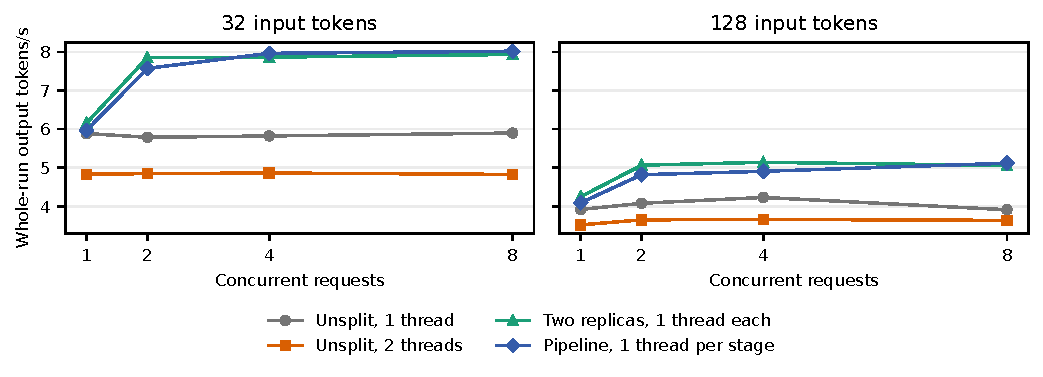
\includegraphics[width=0.94\textwidth]{figures/local-baselines.pdf}
\caption{Observed resource-accounted Qwen3-0.6B throughput on one host, one run per condition. All arms have two available inference CPUs; one-thread unsplit leaves one unused. Coordination uses two other CPUs. No error bars are shown because independent repetitions are absent. Loopback results do not establish multi-machine performance.}
\label{fig:local-baselines}
\end{figure*}

The three-CPU matrix retains two HTTP failures in the replica arm.
Worker 0 exits with SIGTERM during \(Q=8\); one request fails there and
one in the later \(Q=4\) condition reusing that runtime. The signal's
origin was not established. All other conditions return exact reference
outputs. Separate fresh-runtime replica reruns at \(Q=8\) and \(Q=4\)
serve 12 requests without failure and keep all workers alive. These
reruns read saved reference outputs without allocating a reference model
in their driver, changing its memory footprint. They do not prove that
the earlier failures cannot recur, and do not replace failed
observations. Three-worker validation extends functional coverage
without establishing physical heterogeneity or a performance advantage
of the planner.

\hypertarget{replay-correctness-and-stalls}{%
\subsection{Replay correctness and
stalls}\label{replay-correctness-and-stalls}}

All 18 position-controlled recovery cases match the unsplit reference
token sequence, including both active requests where concurrency is two.
This checks 27 request outputs with 16 generated tokens each, not
arbitrary fault schedules. The final sequences contain no duplicated or
omitted tokens relative to that reference. Internally accepted token
times show a maximum gap of 10.005 s in the fresh validation pass. Exact
output is compatible with a substantial user-visible pause.

Relayout waits to reload changed shards; loss reloads the full model on
the survivor; restart rebuilds cache on an unchanged layer layout. Fault
orchestration is manual and explicitly logged. The reported internal
disruption interval begins when the router detects failure; maximum
token gaps also include the orchestration delay. This experiment makes
no claim about automatic detection latency or clients receiving streamed
tokens.

\hypertarget{packaged-application-demonstration}{%
\section{Packaged Application
Demonstration}\label{packaged-application-demonstration}}

The application exposes execution and recovery through a local browser
UI. Its panels show the current layer owner, worker availability,
measured request speed and first-token time, predicted token cost,
controller decisions and a recovery timeline. Chat requests execute the
model on the worker chain. Stop and restore controls terminate or
restart a worker; the controller detects its availability change and
assigns a complete surviving placement.

We launched a Linux amd64 Debian package based on release 0.1.0+ci3
through its packaged launcher, using an isolated application-data
directory. A presentation update replaces the local hostname with CPU
host; worker identifiers and all inference and controller code remain
unchanged. The repackaged version is 0.1.0+ci3.paper2. The launcher
installed its pinned CPU runtime and downloaded Qwen2.5-0.5B-Instruct at
revision \texttt{7ae557604adf67be50417f59c2c2f167def9a775}. This demo
has 24 layers and uses PyTorch 2.14.0 and Transformers 5.17.0. It is a
distinct model, dependency environment and release snapshot from the
Qwen3 research experiments. Running an extracted package payload
verifies its launcher and application, while system-wide installation
through a distribution package manager was not exercised in this
capture.

Fig.\textasciitilde{}\ref{fig:demo-chat} is a fresh browser screenshot
after an actual model answer with two local CPU workers. We then used
the visible Stop w2 control, observed recovery to all 24 layers on w1,
and obtained another model answer. Restoring w2 produced an active split
again. Fig.\textasciitilde{}\ref{fig:demo-recovery} shows captured
placement panels before loss and after recovery. Original screenshots,
execution records, package checksum and capture metadata accompany the
artifact. Both workers run on one host; this sequence does not
demonstrate a second physical laptop joining, benchmark algorithmic
novelty, or prove availability relative to fault-aware replicas. The UI
returns an answer after generation; it is not a client
streaming-delivery check.

\begin{figure*}[t]
\centering
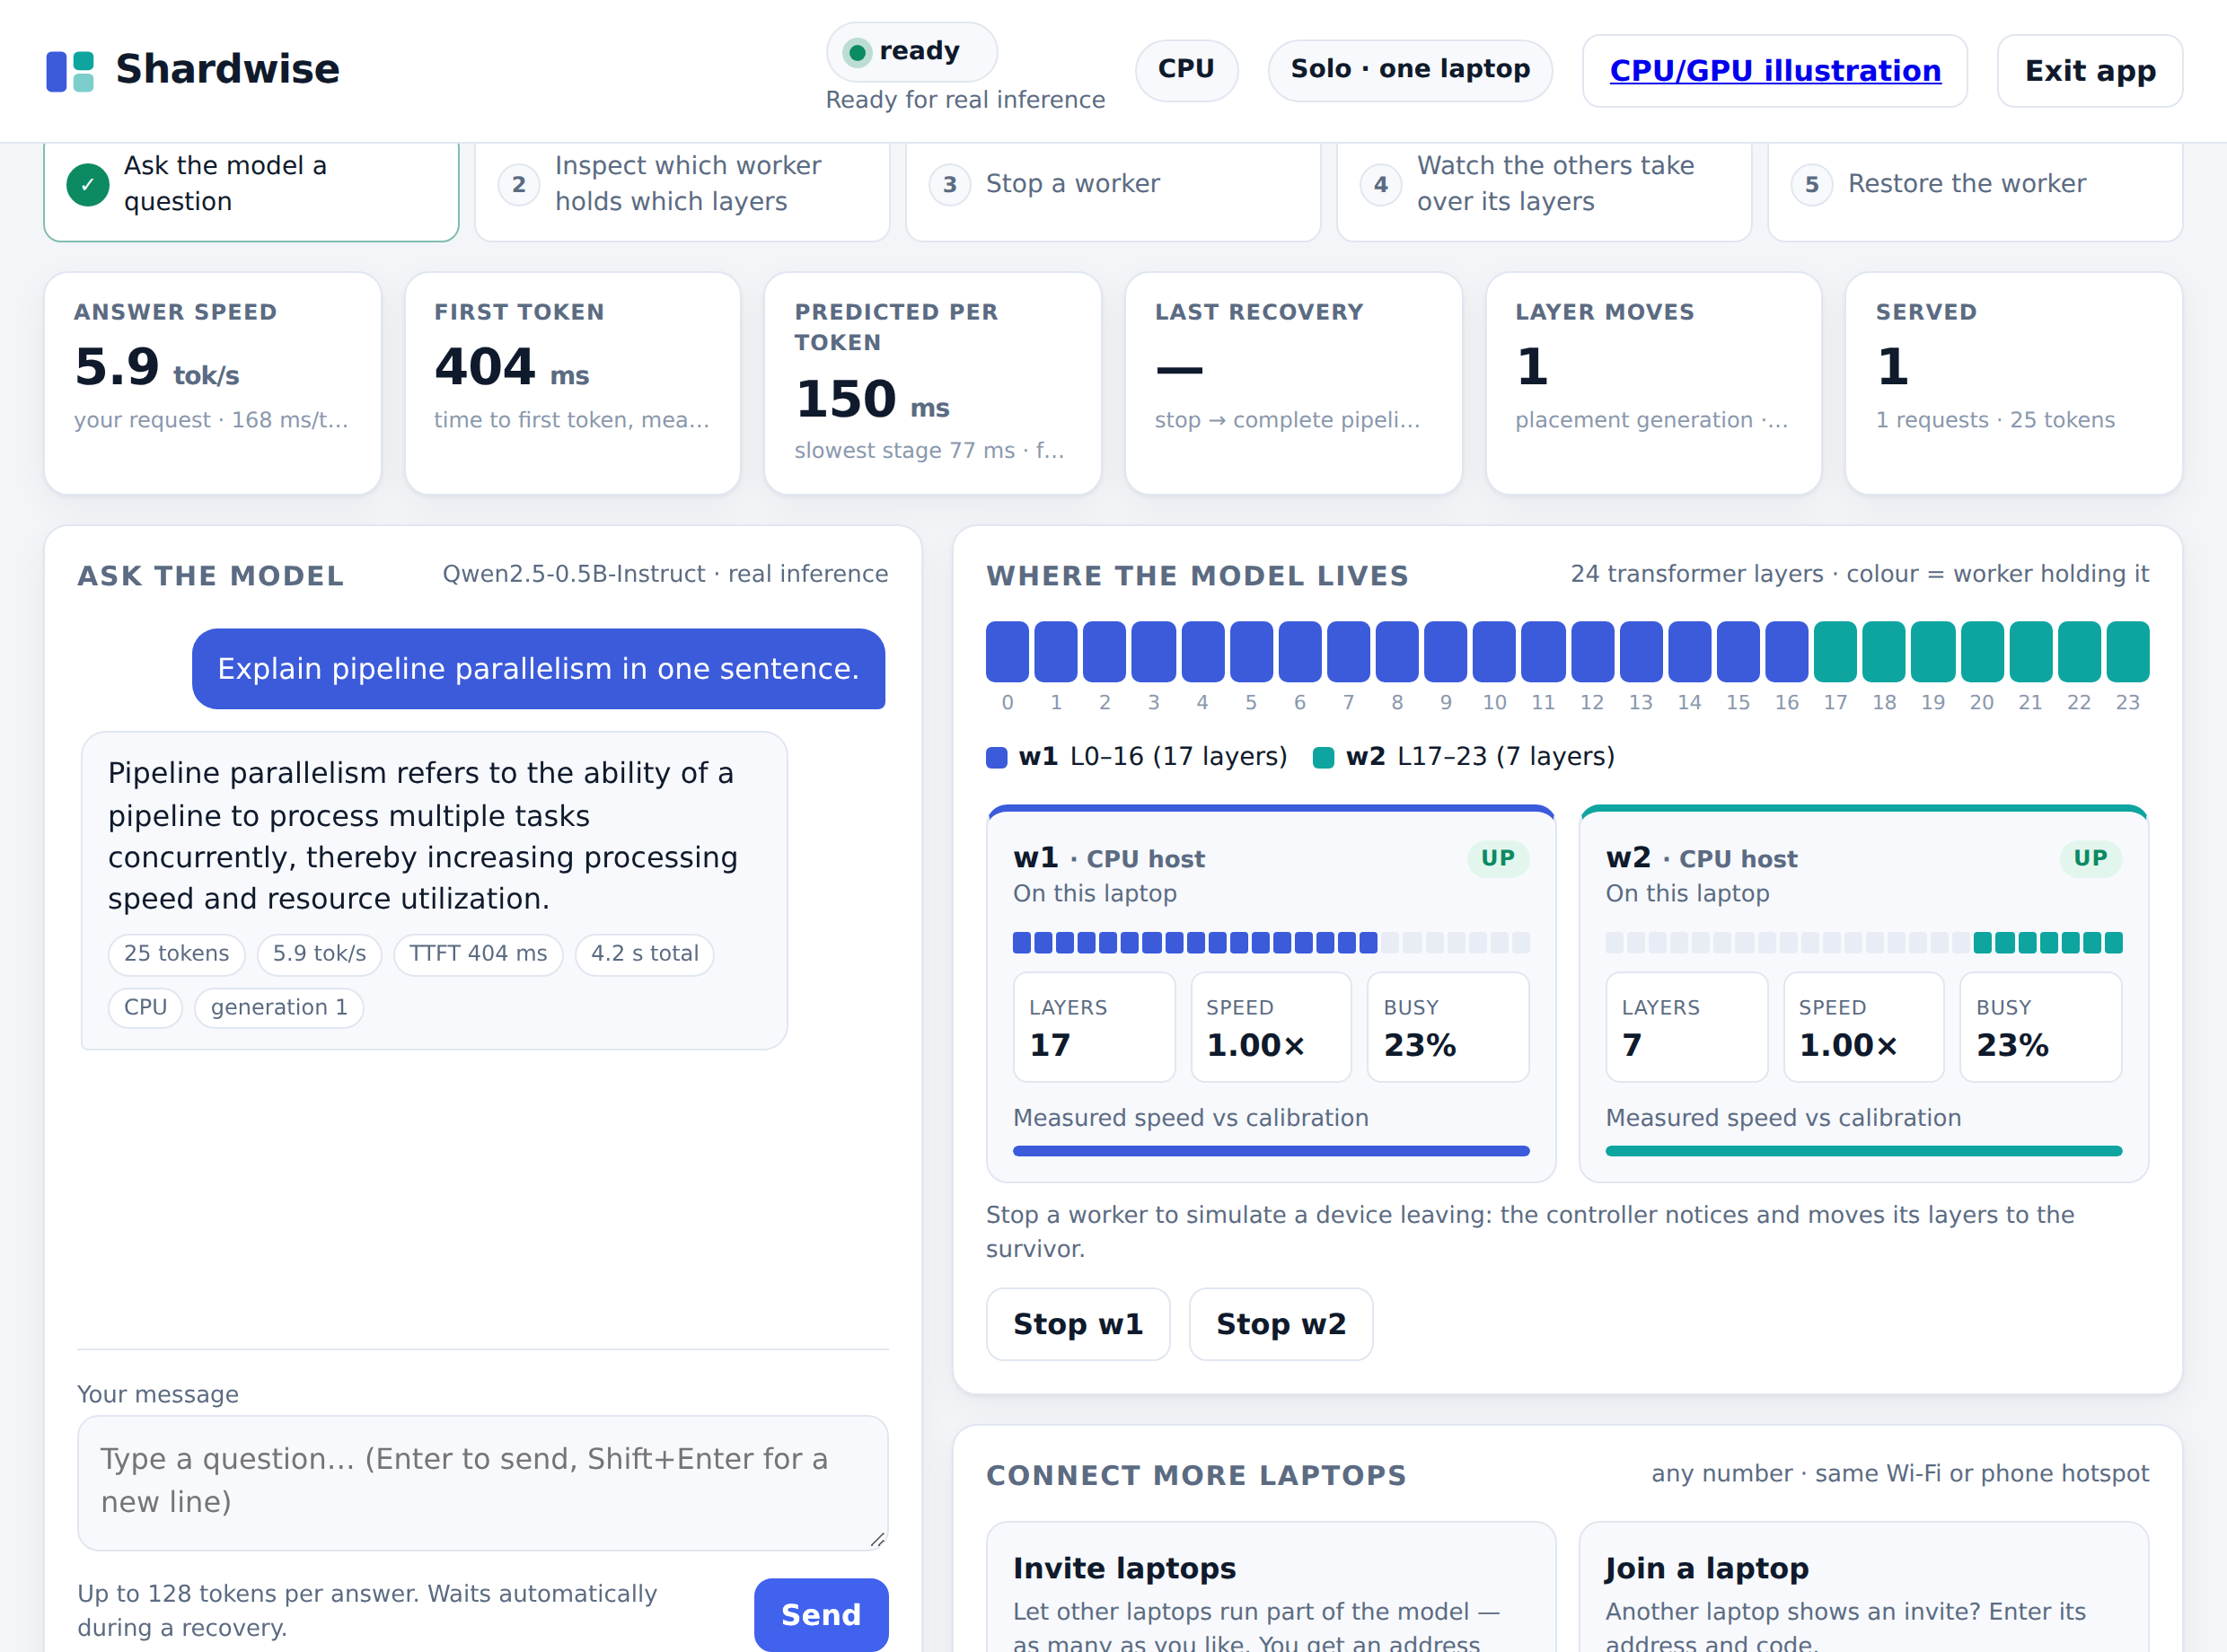
\includegraphics[width=0.96\textwidth]{demo-screenshots/01-real-chat-two-workers.png}
\caption{Actual browser UI from the Debian-packaged application after a real Qwen2.5-0.5B-Instruct answer. Two worker processes on one CPU host hold the 24-layer model. Request measurements belong to this demonstration and are not Qwen3 benchmark results.}
\label{fig:demo-chat}
\end{figure*}

\begin{figure*}[t]
\centering
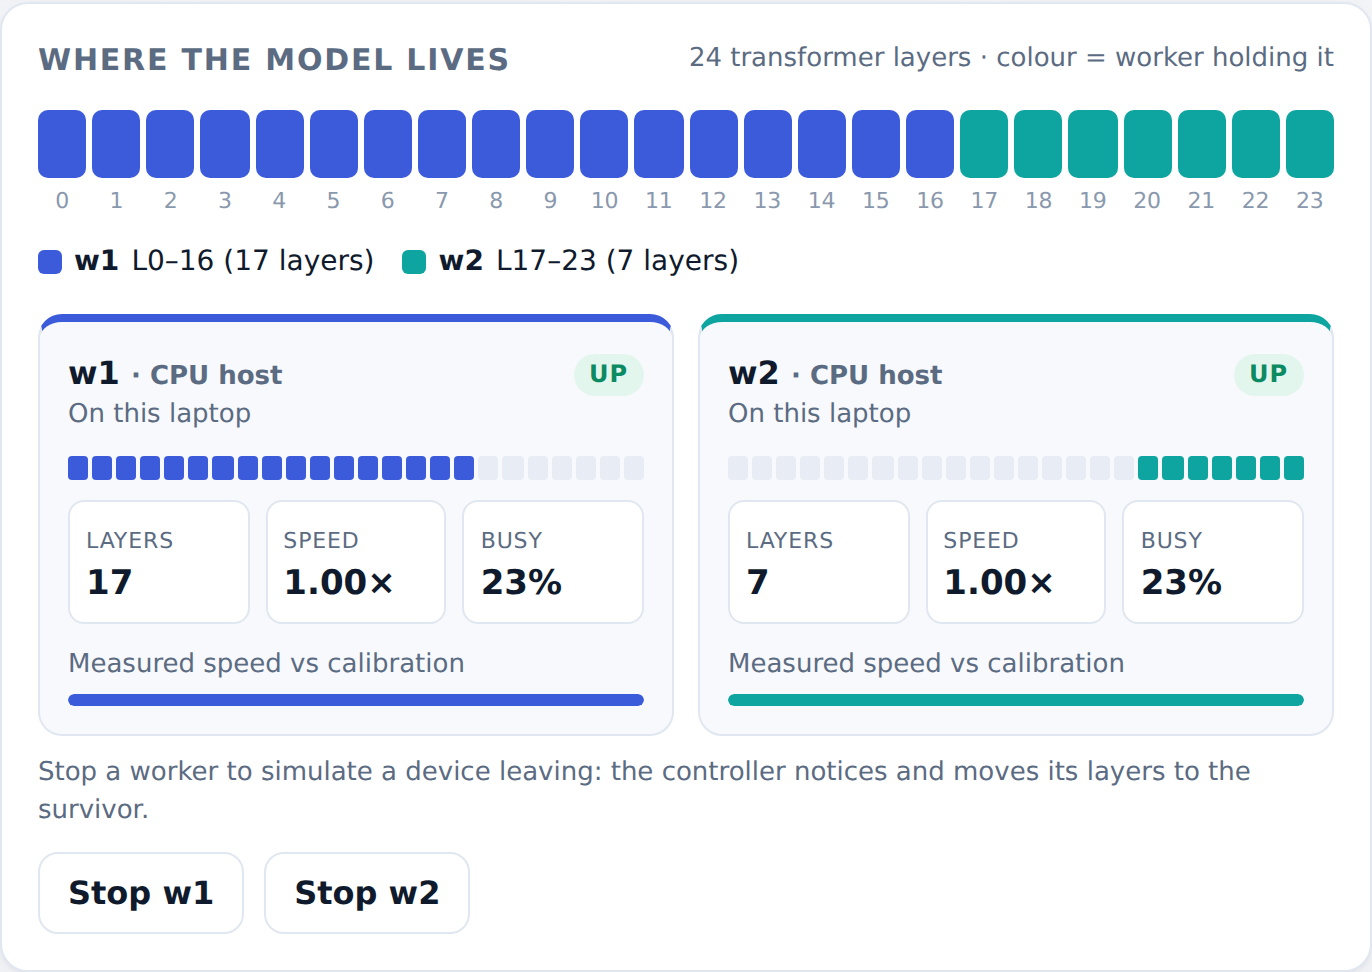
\includegraphics[width=0.48\textwidth]{demo-screenshots/02-two-worker-placement.png}\hfill
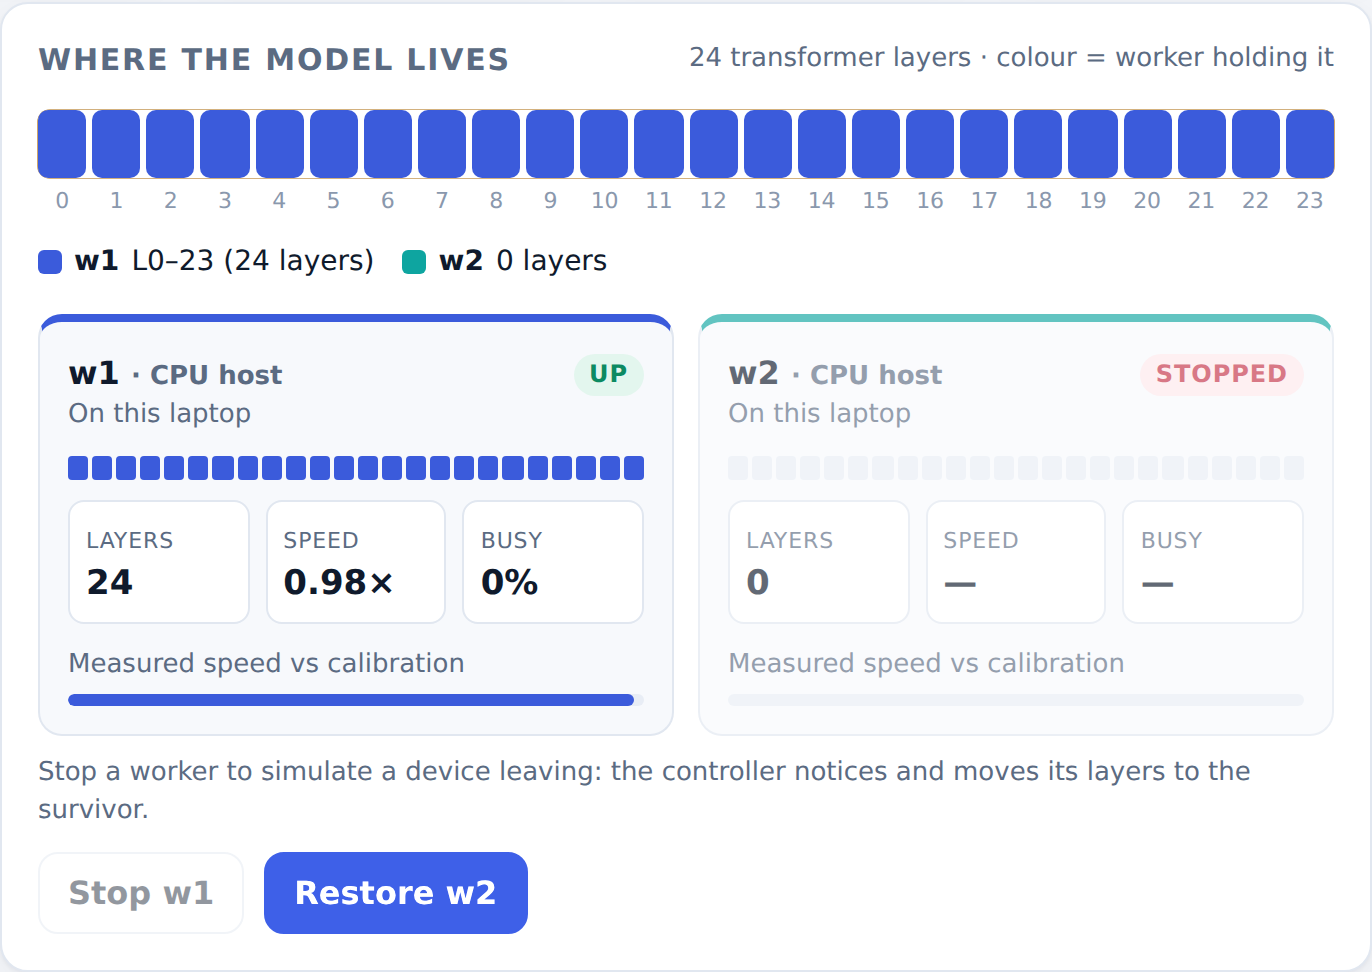
\includegraphics[width=0.48\textwidth]{demo-screenshots/04-recovered-full-model.png}
\caption{Actual placement panels: left, two active workers before loss; right, after the visible Stop w2 action, the surviving w1 holds all 24 layers and w2 is stopped. A subsequent real answer and restored two-worker split were also verified. Screenshots establish execution and control behavior on one host.}
\label{fig:demo-recovery}
\end{figure*}

\hypertarget{illustrative-heterogeneous-configuration}{%
\subsection{Illustrative heterogeneous
configuration}\label{illustrative-heterogeneous-configuration}}

The packaged interface also includes a read-only CPU/GPU illustration
(Fig.\textasciitilde{}\ref{fig:gpu-illustration}). It assigns layers
0--7 to a CPU worker and 8--23 to a GPU worker, illustrating a larger
share for an assumed faster GPU. This is an assumed deployment diagram
shown in the application, not an executed GPU placement, measured
speedup or optimized split. The capture host has no GPU; all execution
and recovery screenshots above are CPU runs. Selecting a real
heterogeneous split requires device-specific compute, endpoint, memory
and transport measurements. No GPU metrics or generated answers are
displayed in the illustrative view.

\begin{figure*}[t]
\centering
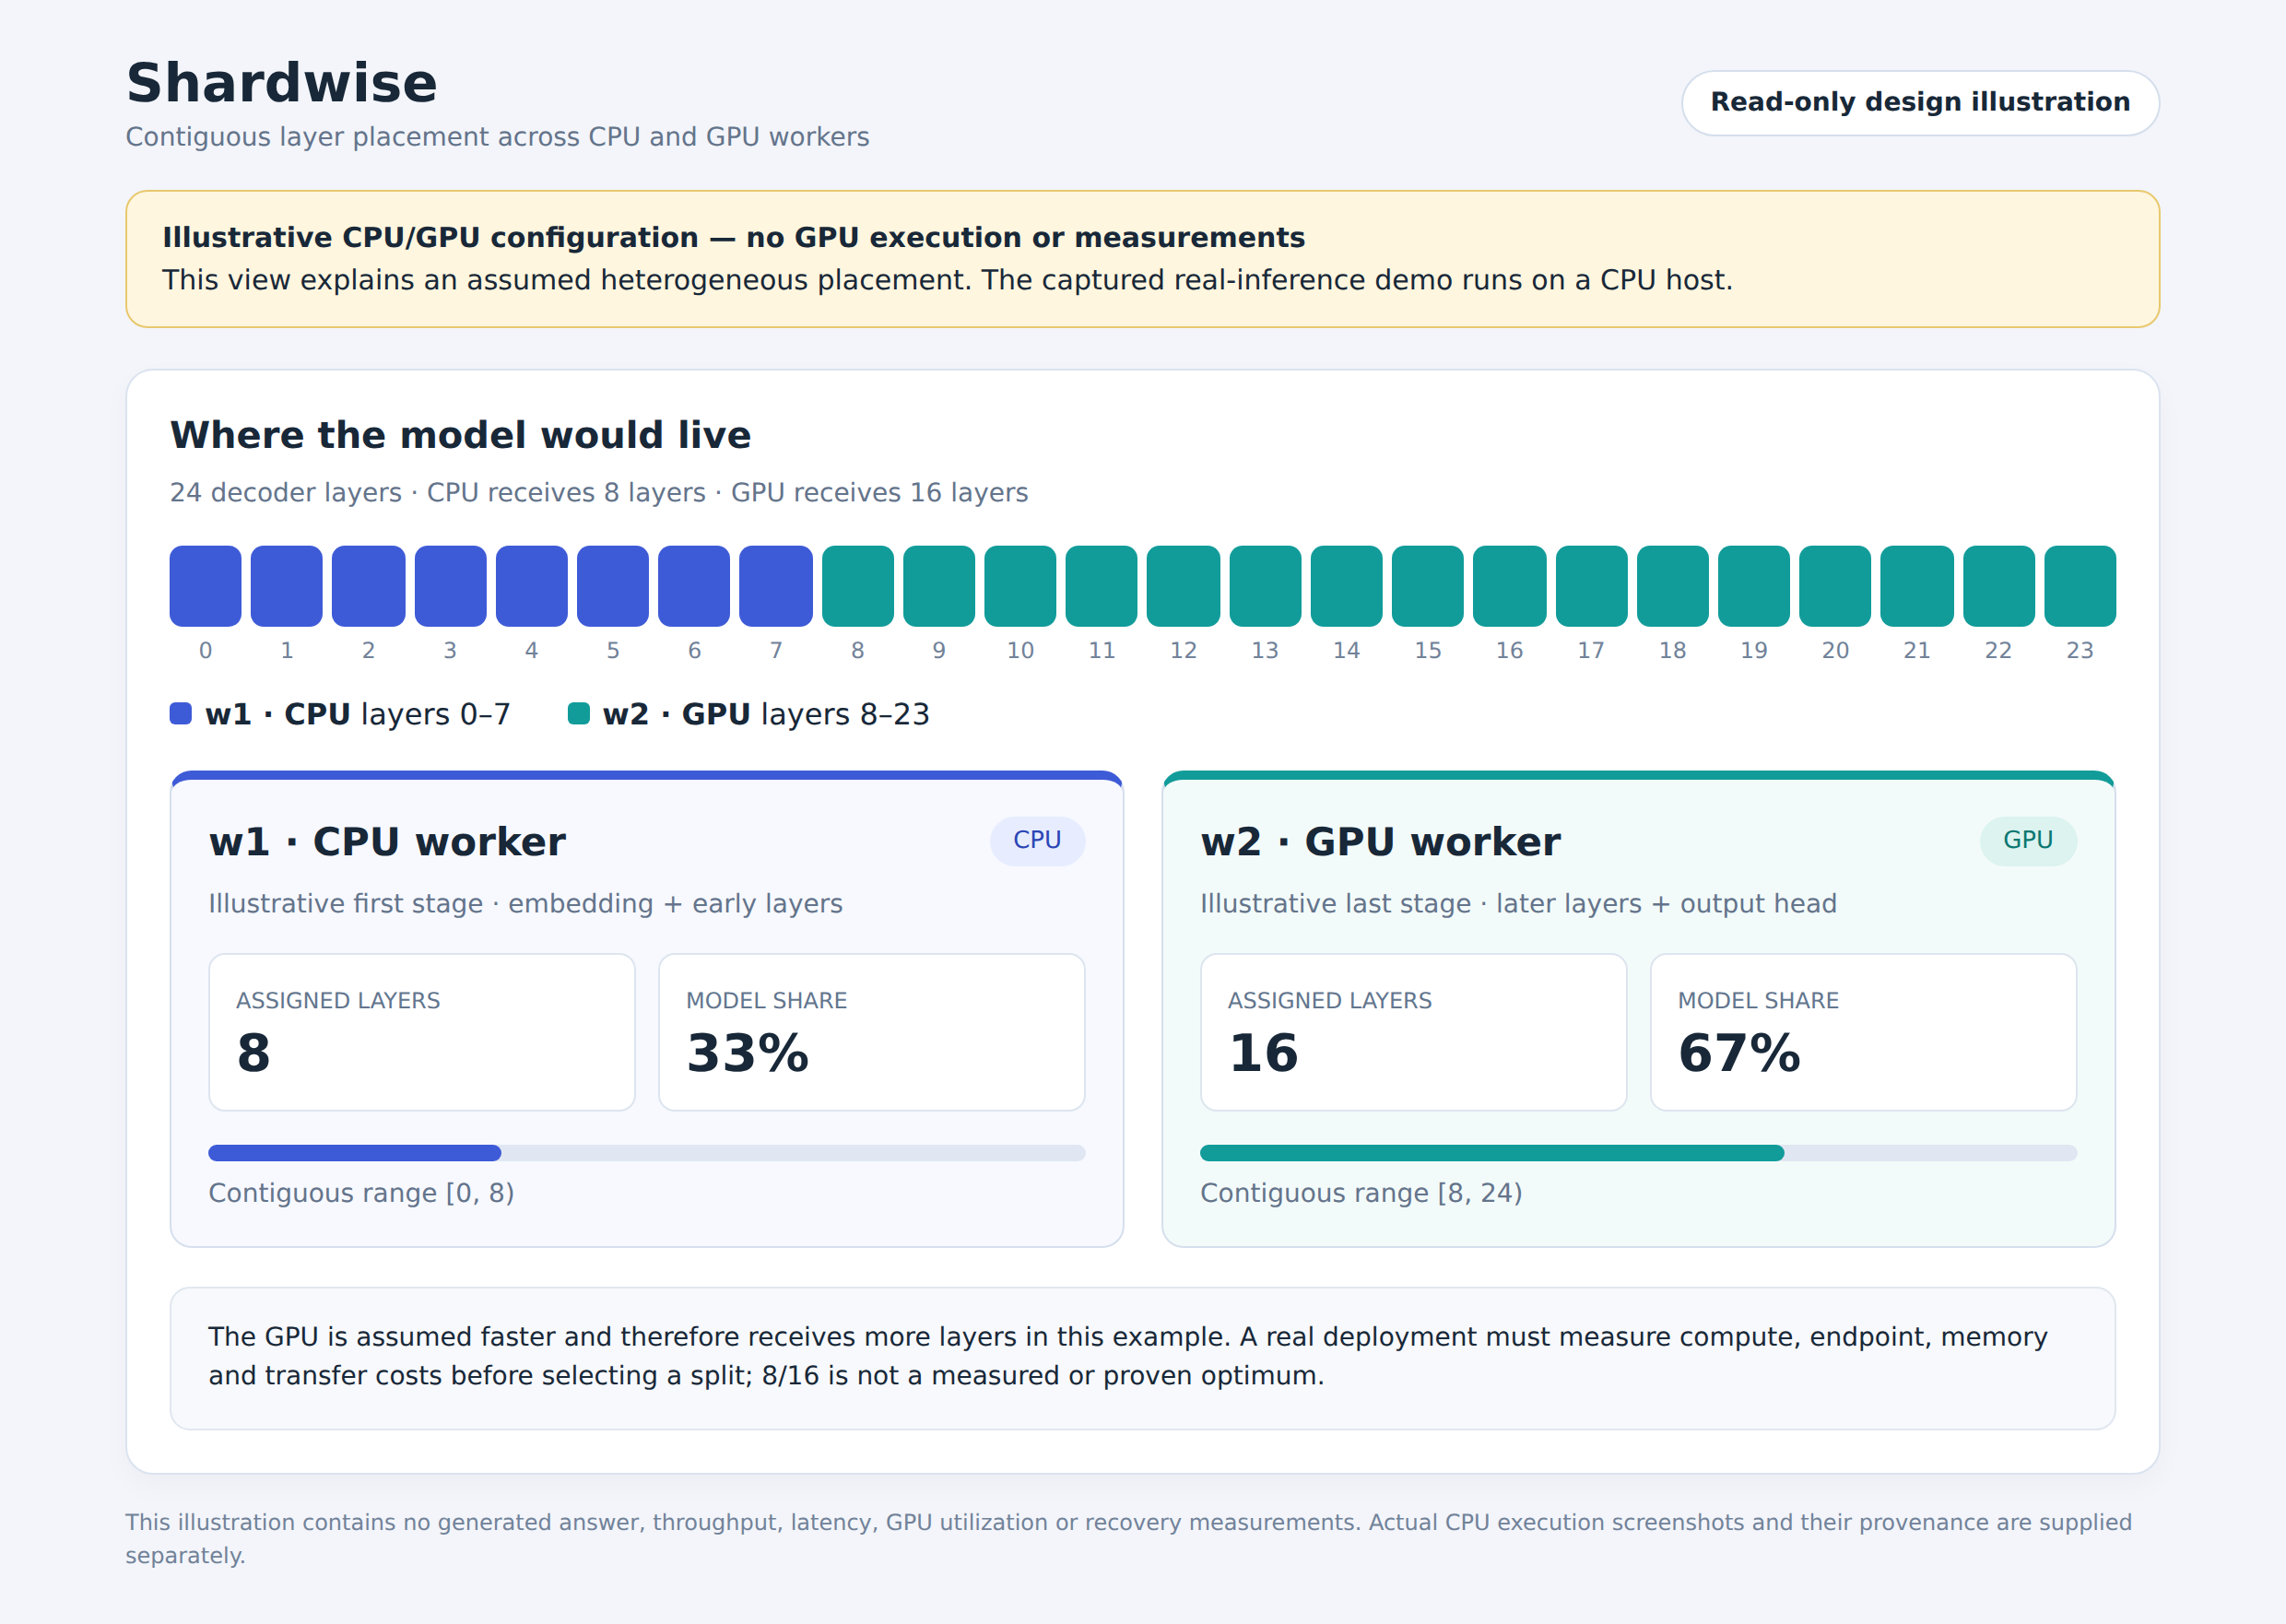
\includegraphics[width=0.96\textwidth]{demo-screenshots/07-cpu-gpu-illustration.png}
\caption{Read-only CPU/GPU illustration in the packaged UI: the CPU worker is assigned 8 layers and the GPU worker 16. The visible banner identifies the view as illustrative; no GPU inference, measurement, or optimal-placement claim is made.}
\label{fig:gpu-illustration}
\end{figure*}

\hypertarget{discussion-and-limits}{%
\section{Discussion and Limits}\label{discussion-and-limits}}

For a model fitting on every worker, replicas and a justified unsplit
CPU configuration should be measured before adopting a pipeline. The
relevant baseline depends on resource budget, precision, dispatch,
batching and model memory. A weak dispatcher can make pipeline overlap
look better than it is. Our replicas use available endpoints, but do not
implement a production batching engine. No state-of-the-art ranking
follows.

Whole-run time is the primary endpoint for short sessions. Reporting
only a fault phase can hide migration, warmup and drain costs. Cost
models must account for every affected history and distinguish serial
replay work from elapsed interruption. A live-context sum and explicit
generation-linked records improve observability; they do not remove
underforecasting or prove an uncertainty-aware controller is better.
Same-generation cache recovery has request-scoped records, because its
global transition identity is not known.

Concurrency changes the useful placement objective, but \(Q>1\) is
insufficient to justify saturation for an arbitrary pipeline. The new
envelope planner fixes an optimization error within the restricted
model. Real-model evidence for three or more physical workers, natural
heterogeneity and controller behavior at changing concurrency remains
necessary.

The historical CPU model is small, prompts and output budgets are short,
machines are similar, and faults are injected. The one-block context and
concurrency matrices extend local functional coverage, but do not
establish repeated results across conditions. Ten restart blocks are a
starting design, not a universal power guarantee; temporal or host
interference can remain. Recovery depends on model-fit and excludes
coordinator loss. The packaged real-inference demonstration is execution
and control evidence; its different model and release are not pooled
with the comparative study.

The strongest next studies are matched-start finite cohorts versus
continuing arrivals, real transport measurements that change placement
decisions, a held-out transition calibration study, an optimized
external serving baseline, additional models, and genuinely different
machines. Negative baseline results should remain in the paper. More
repetitions cannot establish algorithmic novelty or replace missing
deployment conditions.

\hypertarget{conclusion}{%
\section{Conclusion}\label{conclusion}}

The audited two-VM record shows that objective choice, transition
accounting and failure recovery matter, while the payback gate has no
demonstrated advantage over hysteresis. The revised runtime addresses a
finite-concurrency planner error and exposes active replay histories,
queue time and token stalls. Completed position-controlled checks
establish replay correctness only for the tested schedules; the
one-block local checks show why replicas belong in the baseline set,
while leaving stable performance rankings unresolved. This is an
empirical study of conditions and pitfalls, with broader deployment and
external-system comparisons still required.

\hypertarget{artifact-availability}{%
\section{Artifact Availability}\label{artifact-availability}}

The writing bundle contains editable IEEE LaTeX and Markdown, figures,
bibliography, experiment reports, source hashes and build instructions.
The repository preserves historical raw matrices and the new local
measurements separately. A companion application artifact supplies the
verified Debian package, fresh screenshots and capture provenance.
Review access and final author metadata will follow the selected venue's
policy; the anonymous manuscript exposes no author-specific repository
URL.
\bibliographystyle{IEEEtranN}
\bibliography{references}
\end{document}
